\documentclass{beamer}
\RequirePackage[italian]{babel}
\RequirePackage[utf8]{inputenc}

\RequirePackage{amsmath}
\RequirePackage{dsfont}
\RequirePackage{mathtools}
\RequirePackage[linesnumbered,lined,ruled,vlined,commentsnumbered]{algorithm2e}

\RequirePackage[
  backend=bibtex,
  citestyle=authoryear,
  style=alphabetic
]{biblatex}
\addbibresource{bibliography.bib}

\RequirePackage{xcolor}

\RequirePackage{pgfpages}
\setbeamertemplate{note page}[plain]
%\setbeameroption{show notes on second screen=bottom}
%\pdfinfo{/Keywords (SP-Bottom)}

\RequirePackage{minted}
\newcommand{\ipy}[1]{\mintinline{python3}{#1}}

\usetheme{Madrid}
\usecolortheme{seahorse}
\setbeamercovered{transparent}

\RequirePackage{minted}
\usemintedstyle{github}

\RequirePackage{bm}
\renewcommand{\vec}[1]{\bm{#1}}

\RequirePackage[separate-uncertainty = true]{siunitx}

\title[Playing \emph{Connect-4} with DNN]{Playing \emph{Connect-4} with Deep Neural Networks}
\subtitle{}
\author[Luca Arnaboldi]{Luca Arnaboldi}      
\institute[]{Corso ``Computing Methods for Experimental Physics and Data Analysis''}
\date[14-10-2021]{14 ottobre 2021}

\begin{document}
  \frame[plain,noframenumbering]{\titlepage}
  
  \begin{frame}
    \frametitle{Introduzione}
    \begin{columns}
      \column{0.3\textwidth}
        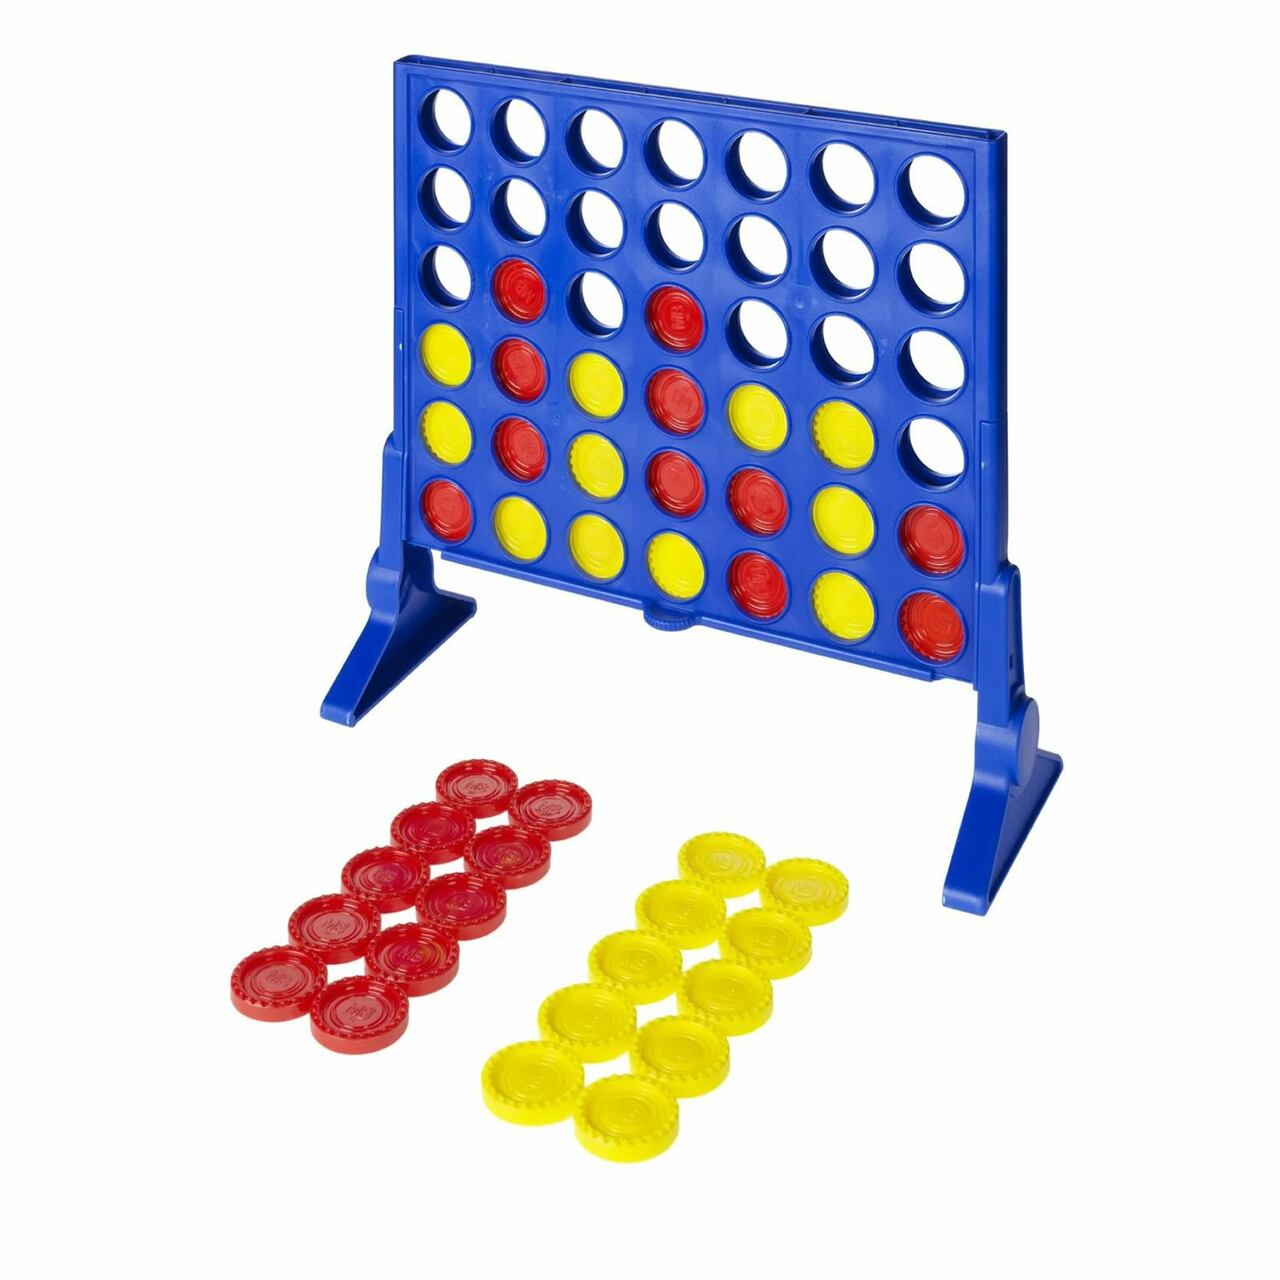
\includegraphics[width=\textwidth]{img/connect4tablegame.jpg}
      
      \column{0.7\textwidth}
        \begin{itemize}
          \item \emph{Forza-4} è un gioco ad informazione completa, con \num{4531985219092} stati possibili \cite{oeis}. 
          \item Il numero di stati limitato permette di risolvere il gioco con algoritmi di ricerca completa.
          \item Non è un problema in cui le reti neurali sono utili ai fini pratici.
        \end{itemize}      
    \end{columns}
    \pause
    È una buona palestra per testare l'abilità delle DNN, potendo fare un confronto con gli algoritmi classici. Seguiamo due approcci:
    \begin{itemize}
      \item \structure{Supervised Learning}: gli algoritmi classici generano il dataset per allenare la rete;
      \item \structure{Reinforcement learning}: il giocatore basato sulla rete neurale gioca contro se stesso ed impara dalle proprie mosse. 
    \end{itemize}
  \end{frame}

  \note{
    ``Questa è veloce una presentazione del progetto, se vogliamo scendere nel dettaglio guardiamo insieme la repo''
  }

  \begin{frame}
    \frametitle{Motore di gioco}
    Ho implementato in \texttt{Python3} il motore di gioco.\\
    Paradigma ad oggetti, uno per ogni componente fondamentale del gioco:
    \begin{itemize}
      \item \ipy{Board}: tavola di gioco, contenente tutti i metodi necessari per aggiungere/togliere pedine, calcolare il vincitore e validare le configurazioni di gioco.
      \item \ipy{Game}: classe che gestisce una partita tra due giocatori. Gestisce l'alternanza dei turni e in generale regola il l'ordine con cui vengono chiamati i metodi sugli oggetti \ipy{Player}.
      \item \ipy{Player}: è la classe classe base per tutti gli altri giocatori; è puramente astratta.
    \end{itemize}
    \pause
    
    Classi Extra: \ipy{Tournament}
  \end{frame}

  \note[itemize]{
    \item \ipy{Tournament} potrebbe implementare calcolo in parallelo.
  }

  \begin{frame}
    \frametitle{Players}
    \begin{itemize}
      \item<1-> \structure{Basic Players}: giocatori senza una vera strategia:
      \begin{itemize}
        \item \ipy{RandomPlayer}: gioca una mossa random tra quelle consentite.
        \item \ipy{ConsolePlayer}: legge dallo \texttt{stdin} le mossa da fare.
        \item \ipy{FixedMovesPlayer}: gioca una sequenza predeterminata di mosse.
      \end{itemize}
    
      \item<2-> \structure{Search Players}: giocatori basati sull'esplorazione dell'albero delle configurazioni. Algoritmo:
      \[\text{minimax} + \text{alpha-beta pruning} + \text{euristiche}\]
      \vspace{-20pt}
      \begin{columns}
      \column{0.05\textwidth}
      \column{0.95\textwidth}
        \begin{block}<3->{\ipy{PerfectPlayer}}
          Implementazione in \texttt{C++} di una ricerca completa\cite{perfectsolvertutotial, perfectsolverimplementation}. Incluso nella repository come submodule.
        \end{block}
      \end{columns}
      \item<4-> \structure{Combination Players}: combinazione di 2 o più giocatori.
      \item<5-> \structure{TensorFlow Players}: valutazione della tavola con un modello di \textit{TensorFlow}.
    \end{itemize}
  \end{frame}

  \note[itemize]{
    \item \ipy{FixedMovesPlayer} è usato principalmente per l'unit testing.
    \item Le euristiche sono l'ordine in un caso e il rumore nell'altro
    \item I giocatori di combinazione sono il \ipy{TwoStagePlayer} e \ipy{PoolPlayer}.
  }

  \begin{frame}
    \frametitle{Extras}
    \begin{itemize}
      \item \structure{Testing}: \texttt{PyTest}
      \item \structure{Linting}: \texttt{Flake8}
      \item \structure{Documentazione}: \texttt{Sphinx}
      \item \structure{Continuous Integration}: \texttt{GitHub Workflows}
      \item \structure{Continuous Deployment}: \texttt{GitHub Pages}  
    \end{itemize}
    \begin{figure}
      
\includegraphics[width=0.8\textwidth]{img/github_badges.png}
    \end{figure}
    \begin{center}
      \url{https://arn4.github.io/connect4/}
    \end{center}
  \end{frame}

  \note{
    ``È una pagina creata in automatico dal README.md''
  }

  \begin{frame}{Codice d'esempio}
  \inputminted[fontsize=\scriptsize]{python3}{code/example-game.py}
  \end{frame}

  \begin{frame}
    \begin{columns}
      \column{0.5\textwidth}
        \centering
        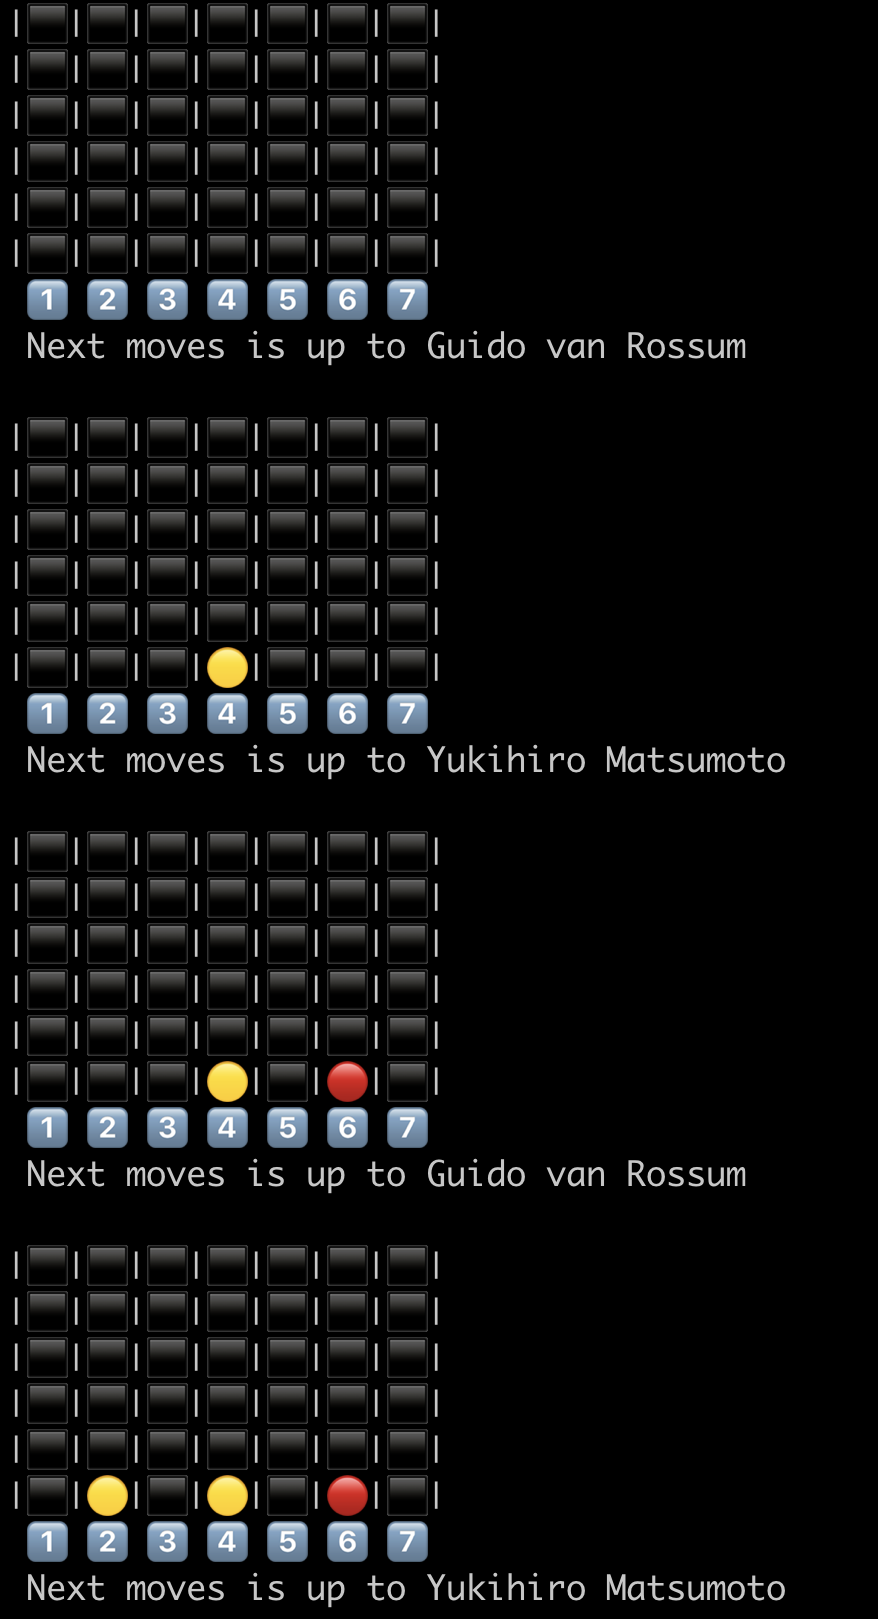
\includegraphics[width=0.8\textwidth]{img/gamestart.png}
      \column{0.5\textwidth}
        \centering
        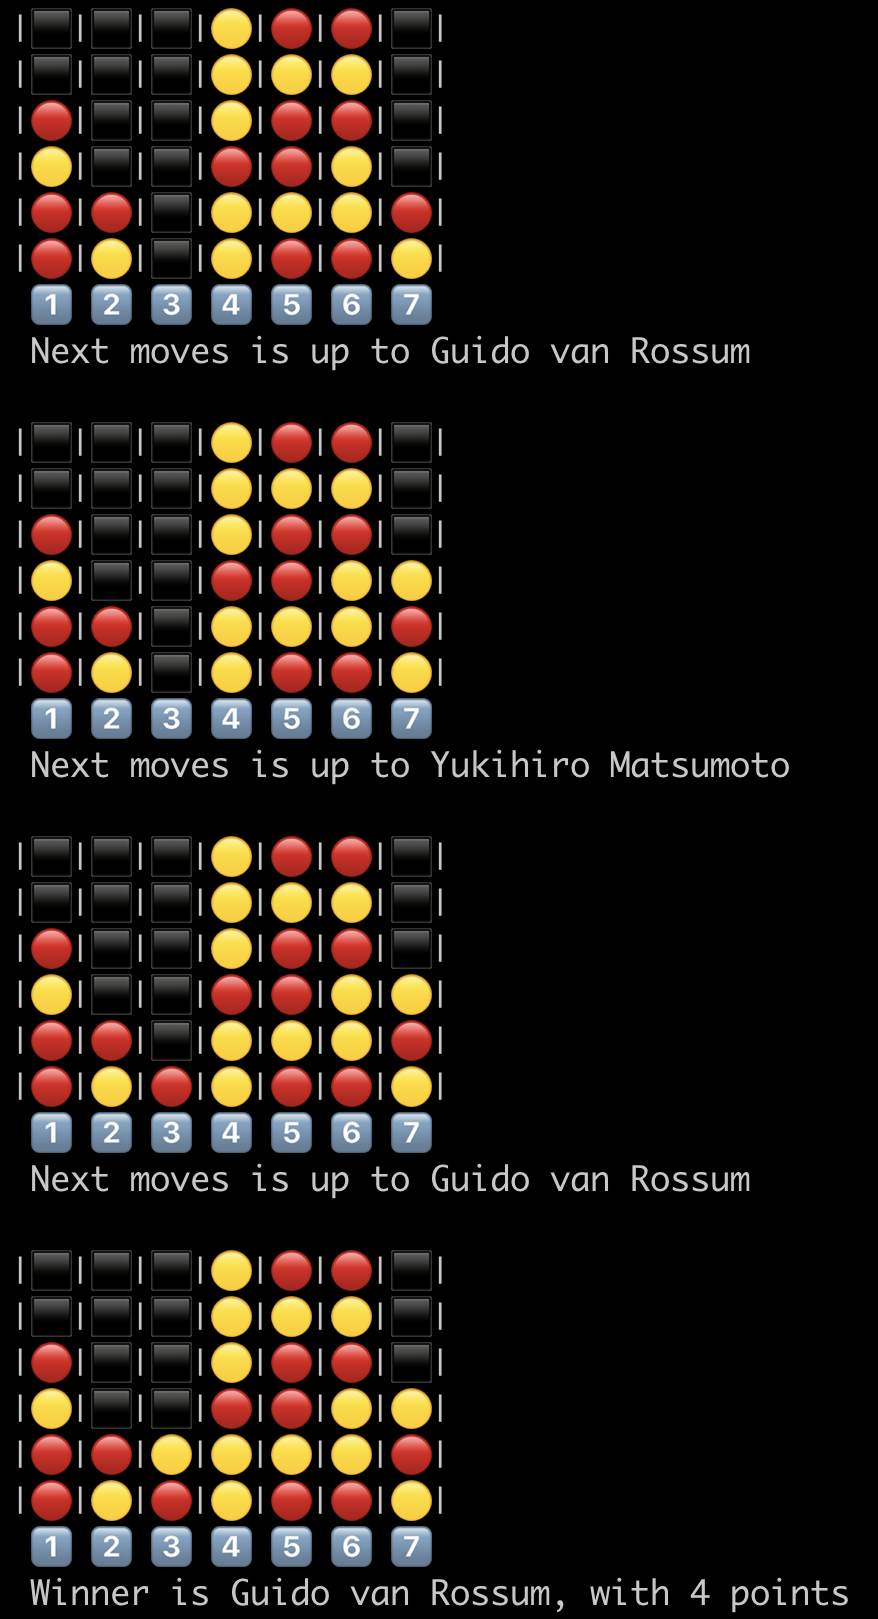
\includegraphics[width=0.8\textwidth]{img/gameend.png}
    \end{columns}
  \end{frame}




  \setbeamertemplate{page number in head/foot}{\phantom{0/0}}
  \begin{frame}[noframenumbering]
    \frametitle{Bibliografia}
    \printbibliography
  \end{frame}
  
\end{document}

